\section{System overview}
\label{sec:system}

This section describes what was built and how the pieces fit together; the
flocking models and the leaders' planner, the parts the experiments compare,
are described in \cref{sec:controllers}. Every choice below was recorded when
it was made, with its reason and the alternatives turned down, in a design
log kept with the code (\texttt{docs/design-log.md}); the section summarises
it.

\subsection{Platform}
\label{sec:platform}

The project runs in Webots R2025a \citep{michel2004}, on its model of the
Bitcraze Crazyflie~2.1, a 10\,cm quadrotor \citep{giernacki2017}. Each drone
runs its own controller, written in Python~3.11; a supervisor, the
\emph{referee}, logs every drone's true position and velocity at every step
for the analysis and takes no part in the flight. The simulation step is
16\,ms.

\paragraph{Why a drone.} Reynolds' boids are point masses: each rule yields
an acceleration, and velocity and position follow from it. A wheeled robot
such as the e-puck, the course's usual robot, cannot behave like that: its
wheel speeds set its velocity directly, with no momentum, and it moves only
where it faces. A quadrotor has inertia and moves in any direction
whatever its heading, so it is the robot closest to a boid
\citep{hauert2011}; it is also the robot real drone flocks are built from
\citep{vasarhelyi2018}. Turned down: a ballbot or a spherical robot, where
balancing or steering would have become the project.

\paragraph{A drone with the real one's limits.} The Webots model is more
capable than the real Crazyflie, so two limits were added to keep the
controllers honest: the motors are capped so that the total thrust is about
twice the weight, as on a real Crazyflie~2.1 (the model's own limit gives over
a hundred times), and the commanded tilt is capped at 30\textdegree.

\paragraph{Flat flight.} All drones fly at one altitude, so the flock moves
in the plane and every obstacle blocks. The code is three-dimensional
throughout, with a single gain switching vertical motion on, but flying over
obstacles was left as future work (\cref{sec:conclusion}).

\subsection{Maps and worlds}
\label{sec:maps}

A map is a small TOML file that describes geometry only: the arena as a union
of axis-aligned rectangles, sector A (the spawn) and sector C (the goal) as
rectangles, and obstacles, walls as boxes and pillars as cylinders, placed by
hand or grown as a seeded forest. The number of drones~$n$, of leaders~$j$ and
the seed belong to the run, not to the map, so one map serves a whole
experiment. A world is generated in four steps, each a pure function tested
without Webots:
\begin{enumerate}
  \item \emph{load} the file into validated data classes (unknown keys are
        rejected with a suggestion, so a typo can't silently change a map);
  \item \emph{build} the course: the arena outline as wall boxes, the
        forests, and checks that need geometry, among them that C can be
        reached from A;
  \item \emph{spawn} the swarm with the run's seed: $n$ drones on the floor
        of A, at a constant density (2\,m$^2$ each, redrawn until they form
        one connected group), and $j$ of them chosen at random as leaders;
  \item \emph{render} the Webots world file.
\end{enumerate}
The obstacle layout has its own seed, in the map, so a change in results can
never come from a different course; the run's seed changes only where the
drones start and which of them lead.

\Cref{fig:maps} shows the three maps of the experiments. \texttt{l\_hall}, a
wide L-shaped hall with a pillar forest before the turn and a wall with a 4\,m
gap after it, is the map the models were developed and tuned on.
\texttt{l\_turn} is the same hall with nothing in it. \texttt{dead\_end} is an
open room with a cup between A and C, open toward A: the straight line from A
to C ends in its bottom, so a leader that steers straight at C leads its flock
into the cup.

\begin{figure}[tbp]
  \centering
  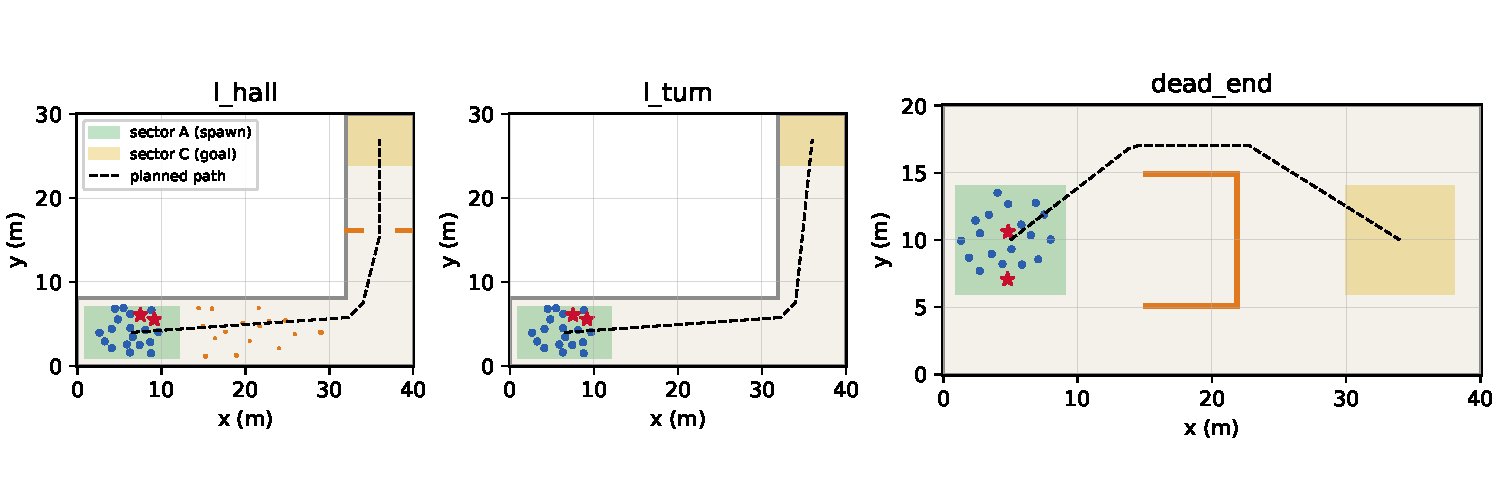
\includegraphics[width=\linewidth]{maps}
  \caption{The maps from above, each with a 20-drone spawn (seed~0):
    followers as dots, the 2 leaders as stars. Grey: the arena's outline;
    orange: obstacles. Dashed: the path the planner finds from A's centre to
    C's (\cref{sec:planner}). \texttt{l\_hall} is the tuning map;
    \texttt{l\_turn} and \texttt{dead\_end} are held out for the evaluation.}
  \label{fig:maps}
\end{figure}

\subsection{The controller's layers}
\label{sec:layers}

Every drone runs the same controller; a leader differs only by knowing where
C is, and by the planning layer that knowledge allows. \Cref{fig:layers}
shows the layers a step goes through.

\begin{figure}[tbp]
  \centering
  % The controller's layers, one step (report/sections/system.tex).
\begin{tikzpicture}[
    node distance=4mm and 6mm,
    layer/.style={draw, rounded corners=2pt, minimum height=8mm, minimum width=26mm,
                  align=center, font=\small, fill=#1},
    layer/.default=white,
    input/.style={align=center, font=\footnotesize},
    flow/.style={-{Stealth[length=2mm]}, thick},
  ]
  \node[layer=blue!8] (sense) {sensing\\[-1pt]\scriptsize IR, GPS, map};
  \node[layer=blue!8, right=of sense] (mission) {mission\\[-1pt]\scriptsize go?\ in C?};
  \node[layer=orange!15, right=of mission] (model) {flocking model\\[-1pt]
                                                   \scriptsize hybrid / Couzin / Reynolds};
  \node[layer=blue!8, right=of model] (limit) {stopping limit};
  \node[layer=blue!8, below=of limit] (velocity) {velocity layer\\[-1pt]
                                                  \scriptsize $(\mathbf v_d-\mathbf v)/\tau$};
  \node[layer=blue!8, left=of velocity] (attitude) {attitude and\\[-1pt]altitude PIDs};
  \node[layer=gray!15, left=of attitude] (motors) {motors};
  \node[layer=red!10, dashed, above=of model] (route) {route (leaders)\\[-1pt]
                                                      \scriptsize plan, pursue, replan};

  \draw[flow] (sense) -- (mission);
  \draw[flow] (mission) -- (model);
  \draw[flow] (model) -- node[above, font=\scriptsize] {$\mathbf v_d$} (limit);
  \draw[flow] (limit) -- (velocity);
  \draw[flow] (velocity) -- node[above, font=\scriptsize] {$\mathbf a$} (attitude);
  \draw[flow] (attitude) -- (motors);
  \draw[flow, dashed] (route) -- node[right, font=\scriptsize] {direction to go} (model);
  \draw[flow, dashed] (sense.north) |- (route.west);
\end{tikzpicture}

  \caption{One control step. Every drone hears its neighbours over infra-red
    and knows its own position and the walls; the flocking model turns that
    into a wanted velocity, which the lower layers fly. Only leaders have the
    route (dashed), which gives the model a direction to C.}
  \label{fig:layers}
\end{figure}

\paragraph{Sensing.} Each drone broadcasts its own velocity, in the world
frame, over an infra-red emitter every step. From each packet it receives, a
drone gets the sender's velocity, its distance (from the signal strength) and
its direction, which is rotated from the tilted body frame into the world
frame. Against the referee's ground truth, distances were off by 1.4\,cm on
average and directions by 0.4\textdegree. The IR carries 3\,m; a drone
considers neighbours within 2.5\,m. Its own position and velocity come from
GPS, and the walls from the map, given to every drone in the world file.
Neighbours are known only from IR and obstacles only from the map, so no
sensor has to correct another.

\paragraph{Mission.} A shared clock starts the trip: the flock forms for the
first 16\,s, all drones hovering by about 6\,s, and then the leaders set
off. A follower does not know where C is, but recognises it when it is inside
(on a real drone, a ground marker; here, GPS against C's rectangle). A drone
in C keeps cruising for 2.5\,m, so the flock fills C instead of piling up at
its edge, and then stops.

\paragraph{Route (leaders only).} At go time a leader plans a path to C on the
map and from then on follows it, planning again if the flock pushes it behind
a wall (\cref{sec:planner}). The route's only output is a direction and a
distance to go, which the model reads exactly as it would read the straight
line to C: with the planning layer off, a leader simply aims at C.

\paragraph{Flocking model.} From what the drone hears, its own velocity, the
mission state and, for a leader, the direction to go, the model computes a
\emph{wanted velocity}. Three models are interchangeable behind one interface
(\cref{sec:models}); everything around them is shared, so the experiments
compare the models and nothing else.

\paragraph{Stopping limit.} Shared by all models, it cuts the wanted velocity
down to what the drone could still brake from before reaching a wall, or a
neighbour, closer than 0.3\,m. It only removes speed, so it cannot push a
drone anywhere; it bounds whatever the model asks for.

\paragraph{Velocity and attitude.} The velocity layer turns the wanted
velocity $\mathbf{v}_d$ into an acceleration
$\mathbf{a} = (\mathbf{v}_d - \mathbf{v})/\tau$, capped at 2.5\,m/s$^2$, with
$\tau = 0.3$\,s, the fastest response measured to have no overshoot. The
acceleration becomes a tilt, which nested angle and rate loops hold as the
Crazyflie firmware does, under an altitude controller and the motor mixing.
\citet{viragh2014} describe a flying robot by exactly these imperfections, a
relaxation time and a maximum acceleration, and \cref{sec:controllers} shows
why they matter: rules that are stable for an ideal boid oscillated on the
drone until the robot could follow them.

\subsection{Choices and why}
\label{sec:choices}

\Cref{tab:choices} lists the choices that shape what the experiments can say,
each with the alternative turned down.

\begin{table}[tbp]
  \centering
  \small
  \begin{tabular}{@{}>{\raggedright\arraybackslash}p{0.27\linewidth}
                     >{\raggedright\arraybackslash}p{0.4\linewidth}
                     >{\raggedright\arraybackslash}p{0.27\linewidth}@{}}
    \toprule
    Choice & Why & Turned down \\
    \midrule
    Followers can't tell leaders from the others &
      Couzin's informed individuals \citep{couzin2005}: the research question
      is what unrecognised leaders can do &
      A leader flag in the IR packet \\
    \addlinespace
    Followers recognise C only when in it &
      Goal recognition, not goal knowledge: they stay uninformed, but a
      flock can stop at C &
      Followers that know C (no leaders needed) \\
    \addlinespace
    Alignment from broadcast velocities &
      A quadrotor flies sideways: its heading says nothing about its motion &
      Alignment with headings \\
    \addlinespace
    Obstacles from the map, position from GPS &
      The Crazyflie's four range rays leave blind spots and see flockmates as
      obstacles; \citet{vasarhelyi2018} also flew among virtual walls &
      On-board range sensing; mapping in flight (a project of its own) \\
    \addlinespace
    Models output a velocity, flown through $\tau$ and $a_{\max}$ &
      The robot is described by two measurable numbers, and every model meets
      the same robot &
      Accelerations straight to tilt \\
    \addlinespace
    Each leader plans on board, for itself &
      A leader that deliberates, from where it is, with what it knows &
      Paths computed by the world generator and handed out \\
    \addlinespace
    Separate seeds for the map and the run &
      Results can't change because the course did &
      One seed for both \\
    \bottomrule
  \end{tabular}
  \caption{Design choices, from the design log.}
  \label{tab:choices}
\end{table}

\subsection{Tools}
\label{sec:tools}

Around the controllers, a small set of tools runs the experiments, all in the
same repository:
\begin{itemize}
  \item \texttt{make\_world.py} builds a world from a map, $n$, $j$ and a
        seed, to open in Webots and watch;
  \item a headless runner starts Webots without a window, runs a world until
        a condition holds, and stops it; an 83\,s run of 10 to 30 drones
        took under a minute of wall-clock time (median 49\,s);
  \item \texttt{sweep.py} runs every combination of $n$, $j$ and seed for a
        model and appends one row per run (time to 90\% in C, drones in C at
        the end, the closest two drones came, crashes, \ldots) to a CSV file;
        a stopped sweep resumes where it left off;
  \item \texttt{tune.py} runs a grid of model settings on seeds kept apart
        from the experiments;
  \item \texttt{analyse.py} computes every number and figure in
        \cref{sec:results} from those files.
\end{itemize}
Any setting of any layer can be changed for one run from the command line,
so an experiment never needs an edited source file. The code (about 3000
lines) is covered by 212 unit tests, checked by a linter and a type checker
on every push.
